\documentclass[10pt,conference,a4paper]{IEEEtran}

\usepackage{amsmath,amssymb}
\usepackage{cite}
\usepackage{algorithm}
\usepackage{algpseudocode}
\usepackage{booktabs}
\usepackage{tabularx}
\usepackage{array}
\usepackage{graphicx}
\usepackage{xcolor}
\usepackage{microtype}
\usepackage{url}
\usepackage{enumitem}
\usepackage{flafter}
\usepackage{placeins}
\usepackage{balance}

\newcolumntype{Y}{>{\raggedright\arraybackslash}X}
\newcommand{\method}{RouteBR}
\setlength{\textfloatsep}{6pt plus 2pt minus 2pt}
\setlength{\floatsep}{5pt plus 2pt minus 2pt}
\setlength{\intextsep}{5pt plus 2pt minus 2pt}

\title{Route Before Response: Fail-Closed Routing for\\
LLM-Enabled Customer-Service Software}

\author{
\IEEEauthorblockN{Yuchen Cao\textsuperscript{1}, Zhenyu Mao\textsuperscript{1}, Jacky Wai Keung\textsuperscript{1},
Yifei Wang\textsuperscript{1}, Guancheng Lin\textsuperscript{1}, Jingyu Zhang\textsuperscript{2,*}}
\IEEEauthorblockA{\textsuperscript{1}City University of Hong Kong, Hong Kong\\
\{cynthcao2-c, zhenyumao2-c, ywang4748-c, guanchlin4-c\}@my.cityu.edu.hk,
Jacky.Keung@cityu.edu.hk}
\IEEEauthorblockA{\textsuperscript{2}Hong Kong Metropolitan University, Hong Kong\\
\textsuperscript{*}Corresponding author: fzhang@hkmu.edu.hk}
}

\begin{document}
\maketitle

\begin{abstract}
LLM-enabled customer-service software can select a semantically plausible service that is inadmissible under the current session, policy, or referenced object. We study this failure as \emph{boundary-aware pre-response routing}. We present \method, a pre-response controller in which one model call commits to a primary action and closed-list object, while deterministic code validates identifiers, evaluates versioned rules, and emits either a typed dispatch or a bounded terminal. Lower-ranked candidates remain diagnostic and cannot replace a blocked primary route. We construct 600 privacy-preserving customer-service scenarios from recurring patterns in confidential requests at a real financial institution; three engineers from the institution jointly reviewed the scenarios and labels. The benchmark combines mixed-service language, paired same-request/different-state cases, and difficult entity references. On the 200-case CONFIRM MAIN split, \method{} reaches 97.5\% final-path exact match, versus 41.0\% for direct routing and 95.5\% for a rule-embedded one-call baseline. Across the 166 bounded cases in CONFIRM MAIN and FLIP, it produces no false dispatch. Removing deterministic state enforcement creates 40 false dispatches in the 40 blocked FLIP cases; removing closed-list object validation blocks all 22 dispatchable ENTITY cases. These results show that a compact proposal--enforcement boundary can improve routing reliability while keeping dispatch authority in deterministic code.
\end{abstract}

\begin{IEEEkeywords}
large language models, query routing, runtime enforcement, entity linking, customer service
\end{IEEEkeywords}

\section{Introduction}

LLM-enabled customer-service software in financial institutions increasingly connects one conversational entry point to information lookup, account analysis, advisory services, support workflows, and protected operations. Tool-augmented language models can interpret open-ended requests and construct calls to external services~\cite{Li2023APIBank,Qin2024ToolLLM,Yao2023ReAct}. These destinations expose distinct interfaces, identifiers, and runtime preconditions. Together, they make the entry point a software integration boundary that passes requests, identifiers, and responsibility to downstream components.

Yet semantic compatibility with a service does not make a route admissible under the current session, policy, or referenced object. Figure~\ref{fig:motivation} fixes the request, history, and referenced object while changing only one permission predicate. One record dispatches the protected action; the otherwise identical record terminates in rejection. The correct downstream path therefore depends on runtime evidence absent from request text.

A routing error at this boundary changes executable software behavior. A wrong action, object, or terminal produces a wrong final path; dispatch under a bounded state is a false dispatch, whereas blocking an admissible path is a false block. Even syntactically valid output may cite an unknown object, use stale state, or miss a higher-priority rule. Engineers must therefore test the complete action--object--terminal contract, separate unsafe dispatch from excessive blocking, and retain the rule or object check behind the outcome. Semantic plausibility alone cannot establish an executable route.

Our evaluation later quantifies this distinction only in the paper's own setting. On the 200-case CONFIRM MAIN split, a direct one-call system obtains 94.0\% action accuracy but only 41.0\% final-path exact match. This scoped result is not an industry prevalence estimate; it shows that high action accuracy can coexist with path failure. We study this problem as \emph{boundary-aware pre-response routing}: from a request and bounded history plus a versioned service catalog, closed object registry, runtime state, and policy rules, the system emits either an admissible action--object dispatch or a bounded terminal. The objective is to preserve flexible language interpretation while making execution authorization reproducible from versioned software records.

\begin{figure}[!t]
\centering
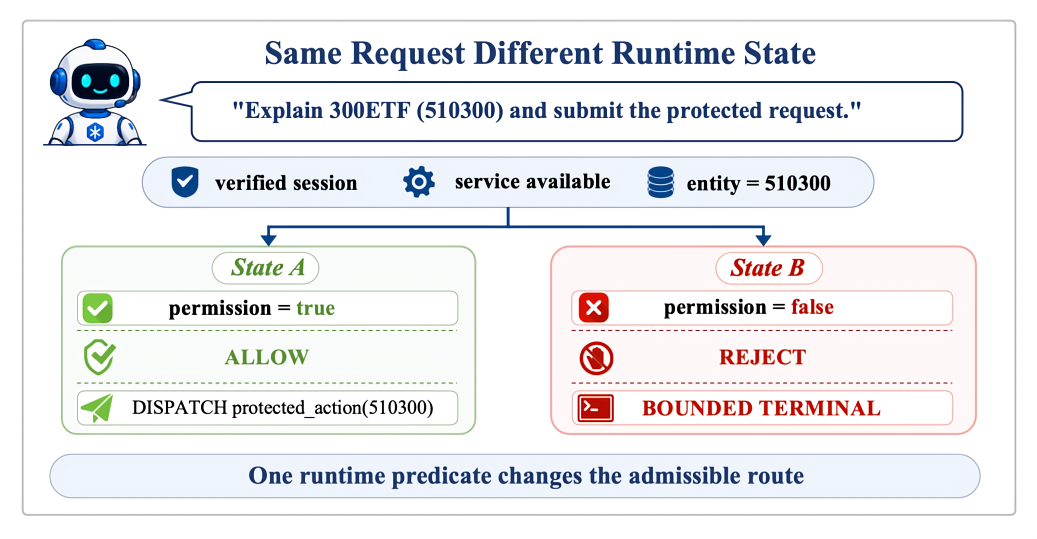
\includegraphics[width=\columnwidth]{figures/routebr_motivating_example_v1.png}
\caption{Motivating state-conditioned route. The request and object are fixed; changing only \texttt{permission} from true to false changes the result from protected-action dispatch to bounded rejection. Semantic match alone does not determine an executable path.}
\label{fig:motivation}
\end{figure}

Adjacent work supplies important parts of this pipeline but usually evaluates a different object. Intent and out-of-scope detection predict labels or abstention; LLM routers select destinations; tool-use studies assess calls and arguments; entity linking resolves identifiers; and runtime controls constrain later transitions~\cite{Larson2019OOS,Hendrickx2024RejectSurvey,Ong2025RouteLLM,Patil2024Gorilla}. Their reported targets leave three composition gaps for the present setting: a semantic action is not a complete action--object--terminal path; a model-predicted boundary does not by itself own execution authorization; and an open-text object mention is not necessarily a dispatchable canonical identifier. Component-level failures can remain hidden even when each local output looks plausible~\cite{Ruan2024ToolEmu,Debenedetti2024AgentDojo,Zhan2024InjecAgent,Xue2025OrchestrationBugs}.

We present \method, which stands for Route Before Response, as a pre-response controller for this boundary. One model call produces a primary semantic action--object proposal. Primary commitment prevents a lower-ranked alternative from replacing a blocked request; deterministic code evaluates versioned state and policy; and a closed-list contract validates the object before emitting a typed dispatch or bounded terminal. Diagnostic alternatives remain audit-only. In this way, semantic selection remains flexible while ordinary code owns the executable transition. Our contributions are:

\begin{itemize}[leftmargin=*,nosep]
  \item We formulate boundary-aware pre-response routing as a state-conditioned, closed action--object decision whose evaluated output is the complete software-visible path.
  \item We design \method, a proposal--enforcement controller that combines primary-route commitment, deterministic state enforcement, closed-list object validation, bounded repair, and replayable traces.
  \item We construct a privacy-preserving benchmark of 600 synthetic reconstructions from recurring confidential-request patterns, jointly reviewed by three engineers from the institution and organized into MAIN, FLIP, and ENTITY cases.
  \item We evaluate complete-path correctness, state-conditioned execution, the closed-list object contract, and backend portability through matched one-call controls, two mechanism removals, and six hosted model backends.
\end{itemize}

\section{Related Work}

\subsection{Customer-Service Task Formulations}

Financial question-answering benchmarks evaluate answers over documents and tables~\cite{Chen2021FinQA,Islam2023FinanceBench}. Task-oriented dialogue represents services through intents, slots, state, and API arguments~\cite{Eric2020MultiWOZ21,Rastogi2020SGD,Byrne2019Taskmaster}; intent, out-of-scope, and selective prediction add labels or abstention~\cite{Casanueva2020Efficient,Larson2019OOS,Geifman2017Selective,Hendrickx2024RejectSurvey}. These tasks motivate service descriptions, history, and bounded refusal, but their target is principally an answer, label, or call inferred from dialogue. Our boundary instead receives runtime state as a separately versioned software record. This permits paired tests in which request-side input is fixed while one predicate and the admissible output change.

\subsection{Semantic Routing and Tool Calling}

Routing research evaluates different output objects. Autoregressive semantic route planning predicts navigation paths from natural-language criteria~\cite{Zhao2024SemanticRouting}, whereas LLM routers select models or services and guarded variants add rejection or prompt-optimized routing behavior~\cite{Ong2025RouteLLM,Sleher2025GuardedRouting,Sleher2026PromptRouting}. Tool-use benchmarks assess interface choice, arguments, execution, or API collections~\cite{Li2023APIBank,Qin2024ToolLLM,Patil2024Gorilla}, while $\tau$-bench combines interaction, tools, policies, and final database state~\cite{Yao2025TauBench}. These studies establish the relevance of routing and policy following. \method{} narrows the evaluated object to one pre-dispatch action--object pair or a bounded terminal. A wrong terminal is a path error, dispatch under a bounded gold state is a safety error, and refusal under \textsc{allow} is an availability error. Table~\ref{tab:positioning} compares these evaluated objects, not the possible extensibility of adjacent systems.

The distinction also changes the oracle. Router evaluation commonly asks whether the selected destination is appropriate, while tool-use evaluation may continue through arguments, execution, and task outcome. Our controller ends earlier but requires a stronger precondition at that point: the selected action, canonical object, versioned state, and terminal must agree before any response service is invoked. A correct bounded terminal cannot erase a wrong semantic action from diagnosis, and a correct action cannot compensate for dispatch under a prohibiting state. This contract-level oracle motivates reporting path, false-dispatch, and false-block measures together rather than treating routing as destination accuracy alone.

\subsection{Entity Linking and Runtime Control}

Named-entity recognition identifies spans and types; entity linking maps mentions to canonical identifiers~\cite{Tedeschi2022MultiNERD,Wu2020BLINK,DeCao2021GENRE,DeCao2022mGENRE,Botha2020Entity100}. \method{} uses a smaller closed-list problem: the supplied registry defines the only dispatchable objects, and ambiguity becomes \textsc{unresolved}. Runtime rails, adaptive guards, and executable specifications separately constrain model-driven transitions~\cite{Rebedea2023NeMo,Yang2025AdaptiveGuard,Wang2025AgentSpec}. \method{} joins these restrictions after semantic selection: code checks the committed action against state and its object against the catalog before invocation. A trace can therefore attribute a bounded path to a named rule, unresolved object, or persistent interface failure rather than to a generic refusal. This scope is narrower than general NER or agent safety, but directly testable at a software dispatch boundary.

Closed-list linking is not used here as a general information-extraction claim. The registry is an interface asset supplied for the current request, and the relevant question is whether a proposed identifier is both canonical and permitted by the selected action contract. An out-of-registry string is therefore not merely a linking error; if allowed to cross the boundary, it becomes an invalid downstream argument. Conversely, resolving every ambiguity by refusal can be safe but unavailable. This connection between canonical identity and dispatchability is why RQ3 evaluates object accuracy together with final path and false block.

Table~\ref{tab:positioning} compares evaluated objects rather than hypothetical extensibility. A check means that the cited formulation explicitly evaluates the property; a cross means that the property lies outside its reported evaluation target. Boundary-aware pre-response routing combines the closed object, versioned state, typed action contract, deterministic transition owner, and paired state test in one pre-dispatch decision.

\begin{table}[!t]
\caption{Representative formulations and evaluated properties. Obj.: closed object; State: runtime predicates; Typed: action contract; Code: deterministic transition owner; Flip: paired state test.}
\label{tab:positioning}
\centering
\footnotesize
\setlength{\tabcolsep}{1.2pt}
\renewcommand{\arraystretch}{1.27}
\begin{tabularx}{\columnwidth}{@{}Y>{\raggedright\arraybackslash}p{0.17\columnwidth}ccccc@{}}
\toprule
Formulation & Output & Obj. & State & Typed & Code & Flip \\
\midrule
Intent/OOS~\cite{Casanueva2020Efficient,Larson2019OOS} & Label/reject & $\times$ & $\times$ & $\times$ & $\times$ & $\times$ \\
Entity linking~\cite{Wu2020BLINK,DeCao2021GENRE} & Canonical ID & \checkmark & $\times$ & $\times$ & $\times$ & $\times$ \\
LLM routing~\cite{Ong2025RouteLLM} & Destination & $\times$ & $\times$ & $\times$ & $\times$ & $\times$ \\
Guarded routing~\cite{Sleher2025GuardedRouting} & Service/reject & $\times$ & $\times$ & $\times$ & $\times$ & $\times$ \\
Tool use~\cite{Li2023APIBank,Qin2024ToolLLM,Patil2024Gorilla} & Tool call & $\times$ & $\times$ & \checkmark & $\times$ & $\times$ \\
Runtime control~\cite{Wang2025AgentSpec} & Transition & $\times$ & \checkmark & \checkmark & \checkmark & $\times$ \\
\textbf{Pre-response routing} & Action pair & \checkmark & \checkmark & \checkmark & \checkmark & \checkmark \\
\bottomrule
\end{tabularx}
\end{table}

\FloatBarrier
The comparison identifies a composition gap rather than claiming that adjacent systems cannot be extended. Dialogue models supply request-side structure, routers supply candidate destinations, entity linkers supply canonical identifiers, and runtime-control work supplies executable guards. Boundary-aware pre-response routing makes their handoff the evaluated object: the semantic stage commits to one current action, the object remains inside a supplied registry, and code reproduces the state transition from versioned inputs. Its regression oracle must therefore preserve the relation among action, object, state, and terminal. Testing only the action can accept an unsafe dispatch, while testing only the terminal can conceal a wrong but conservatively blocked route.

\section{\method}
\label{sec:routebr}

\subsection{Overview and Formulation}

Figure~\ref{fig:overview} places \method{} between a customer entry point and downstream response services. Its input is $I=\langle x,h,\mathcal{S},\mathcal{E},z,\mathcal{R}\rangle$: request $x$, bounded history $h$, versioned service catalog $\mathcal{S}$, closed entity registry $\mathcal{E}$, runtime state $z$, and prioritized rules $\mathcal{R}$. The output is either a dispatch record $(a,o)$ or one terminal in $\{\textsc{clarify},\textsc{defer},\textsc{handoff},\textsc{reject}\}$. Customer-facing response generation is outside this boundary.

The trust boundary separates three owners. Product engineers own the catalog and the versioned rule set; the session and service infrastructure own $z$; the model contributes only a typed semantic proposal. A downstream response service is not addressable from the model adapter. It can be reached only through the controller's dispatch return, after all contracts have succeeded. Consequently, a parseable model output is evidence for semantic selection, not authorization. This division also makes configuration changes local: a new rule version can alter admissibility without changing the prompt, whereas a catalog change can be reviewed as an interface migration.

\begin{figure*}[!t]
\centering
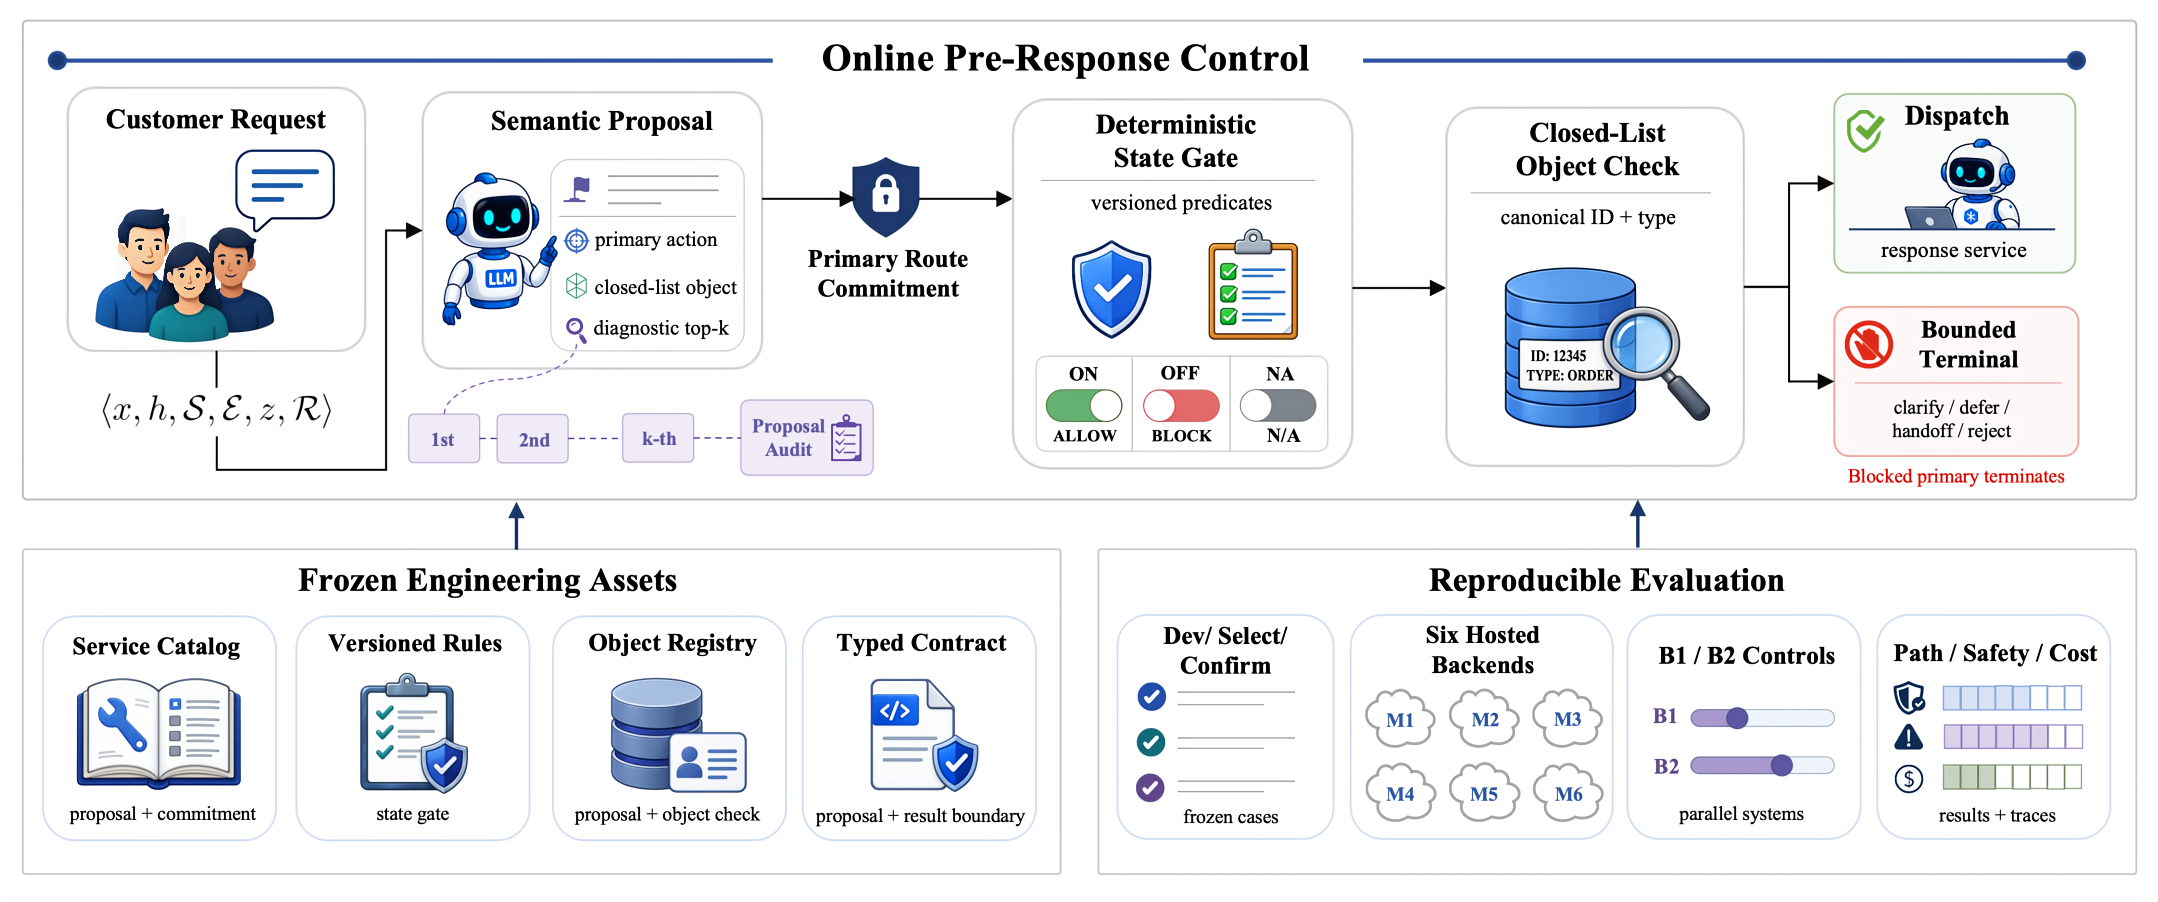
\includegraphics[width=\textwidth]{figures/routebr_overview.png}
\caption{\method{} execution and evaluation framework. The online path commits to one semantic proposal, then code applies state and object checks before dispatch or a bounded terminal; lower-ranked candidates remain audit-only. Frozen assets feed their corresponding control points, not the customer-request card. Evaluation wraps and measures the controller rather than entering its online path.}
\label{fig:overview}
\end{figure*}

The lower panels are dependencies and evaluation, not online stages. Frozen assets map to distinct control points: the catalog constrains proposal and action validation; rules drive the state gate; the registry supplies candidates and the closed-list check; and the typed contract validates proposal and result records. The catalog has five action families with stable identifiers and permitted object types; eight synthetic predicates and prioritized rules with a default \textsc{allow} model the boundary without reproducing institutional policy. Evaluation wraps the controller: DEV, SELECT, and CONFIRM supply cases, backends replace only the proposer, B1 and B2 run in parallel, and path, safety, and cost metrics consume final results and traces.

Table~\ref{tab:catalog} summarizes the interface surface. The names describe response-service families, not customer-visible business units. Four actions are object-sensitive, while support can be object-free. This difference is encoded in the catalog rather than inferred after routing. A protected action is not special-cased in the model prompt; its additional identity and permission requirements are ordinary policy rules evaluated only after it becomes the committed primary action.

\begin{table}[!b]
\caption{Closed action contracts used by \method. All identifiers are versioned catalog values.}
\label{tab:catalog}
\centering
\footnotesize
\setlength{\tabcolsep}{2.4pt}
\renewcommand{\arraystretch}{1.13}
\begin{tabular}{@{}lll@{}}
\toprule
ID & Response-service family & Permitted object type \\
\midrule
A1 & Advisory & ETF \\
A2 & Information lookup & ETF or topic \\
A3 & Account analysis & Account or ETF \\
A4 & Support & None or service \\
A5 & Protected action & ETF or account \\
\bottomrule
\end{tabular}
\end{table}

The model produces $q=\langle a,o,K\rangle$, where $a\in\mathcal{S}$ is the primary action, $o\in\mathcal{E}\cup\{\textsc{none},\textsc{unresolved}\}$, and $K$ contains at most three unique catalog actions. The contract requires $a=K_1$. This equality turns ranking into an executable commitment: $K_2$ and $K_3$ are retained for audit, but never become fallback routes after policy evaluation.

We define a final path as the pair of an executable action and object when the terminal is \textsc{dispatch}, or as one bounded terminal otherwise. Exact-match evaluation therefore compares the software-visible result, not an internal ranking. Two proposals with the same action can differ in final path because their objects differ; two identical proposals can also produce different final paths because $z$ selects different policy outcomes. This definition is what links semantic routing to the integration contract exercised by the experiments.

Figure~\ref{fig:motivation} illustrates the resulting composition. Both records provide the same request, history, catalog entry, and canonical ETF. The proposal contract should therefore produce the same protected-action pair. The state gate then reads the only changed field, \texttt{permission}, and selects either the named \textsc{allow} rule or the bounded \textsc{reject} rule. Only the former reaches the object contract and dispatch return. The example is intentionally small: it does not claim that one predicate represents an institutional workflow. It defines a regression shape in which semantic evidence is held fixed, a versioned runtime fact changes, and the expected software path changes with it.

This decomposition yields three independently testable interfaces. The proposal interface accepts only catalog and registry identifiers. The enforcement interface accepts an already validated primary action plus a state and rule version, and returns a named boundary decision. The dispatch interface accepts only an \textsc{allow} result and a validated action--object pair. A release can therefore replay policy and object checks from a stored proposal without calling the hosted model. Conversely, prompt or backend changes can be tested against frozen state and policy assets. The implementation and evaluation use these seams to separate semantic, state, object-validation, and adapter errors rather than assigning every wrong path to the model.

\subsection{Proposal and Primary Commitment}

The prompt receives request text, dialogue history, catalog descriptions, and candidate entities, but not runtime predicates or rules. It selects the current requested function rather than a hypothetical later action, and resolves an object only through exact code, name, alias, or unique antecedent evidence. The prompt returns one JSON object with \texttt{action\_id}, \texttt{object\_id}, and \texttt{topk}. This separation prevents the semantic call from adapting its preferred action to whatever runtime route happens to be allowed.

The prompt uses the catalog and entity arrays as data, not instructions. It gives priority to a complete current request with an explicit object or imperative expression; emotional language, conditional future operations, and supporting explanations remain secondary cues. For object resolution, exact codes and aliases precede display names and a unique antecedent in the bounded history. Similarity matching and generated identifiers are forbidden. These constraints do not guarantee a correct proposal, but they make every accepted value checkable against the supplied interface.

The validator rejects unknown or duplicated actions, disagreement between the primary action and $K_1$, out-of-registry objects, and object types incompatible with the primary action. It permits one format-only repair that receives the invalid output and validation errors but may not replace semantic evidence or closed identifiers. A second failure reaches a configured non-dispatch terminal. The accepted proposal and every validation error remain in the trace.

Validation proceeds from syntax to enumerated identifiers and then to cross-field relations. This order separates a malformed provider response from an unknown catalog value, and separates both from an object whose type is incompatible with an otherwise valid action. The trace retains the first failed contract and the supplied value rather than only the eventual terminal. As a result, fail-closed behavior does not erase the maintenance signal: adapter owners can investigate schema failures, catalog owners can inspect action errors, and registry owners can review unresolved or mistyped objects without inferring the cause from a generic refusal.

Repair is deliberately narrower than a second routing attempt. The original payload, invalid output, and error list are preserved, and the repair instruction asks only for a contract-conforming representation of the same semantic choice. This prevents repeated calls from searching for an action that happens to pass the policy. If the corrected object still lies outside $\mathcal{E}$, if the primary action changes, or if the output again violates the schema, the controller terminates. The experiments count repair as an additional API call and report first-pass JSON validity separately.

Primary commitment is the key compositional invariant. Suppose the request supports a protected action and an advisory alternative. If the protected action is primary but current permission is false, the controller returns the rule's terminal. It does not reinterpret the lower-ranked advisory candidate as an executable substitute. This prevents semantic ranking from becoming an implicit policy-bypass mechanism.

This invariant also clarifies responsibility for mixed-service language. The model must choose which function is current and primary; the policy engine decides only whether that action is admissible. The engine does not rank semantics, and the model does not search the policy space. A wrong primary action remains a measurable semantic error rather than being concealed by a later fallback. Diagnostic alternatives can still help engineers inspect ambiguity or revise catalog descriptions, but they have no execution authority.

\subsection{Deterministic Enforcement and Object Validation}

For the committed action $a$, the policy engine selects the first matching rule:
\begin{equation}
b(a,z,\mathcal{R})=r_j.\mathrm{decision},\quad
j=\arg\min_{i:r_i(a,z)=\mathrm{true}} r_i.\mathrm{priority}.
\end{equation}
The model does not predict $b$ and cannot override it. If $b\neq\textsc{allow}$, \method{} records the winning rule and returns the corresponding terminal. The state-removal intervention in RQ2 bypasses this transition while keeping the same semantic proposal, exposing the errors prevented by code-owned policy.

Rules are ordered by numeric priority and then stable rule identifier. The study uses eight non-default predicates: safety escalation, unsupported request, service unavailability, unclear scope, unresolved entity state, unverified identity, missing protected-action permission, and stale context. A final empty-condition rule returns \textsc{allow}, making the policy function total for every catalog action. This explicit default is important for replay: absence of a matching prohibition is represented by a named rule rather than by missing control flow.

When $b=\textsc{allow}$, the object contract checks whether $a$ requires an object, whether $o$ belongs to the supplied registry, and whether its type is permitted by the catalog. An unresolved required object returns \textsc{clarify}; object-free support paths require \textsc{none}. The closed-resolver intervention in RQ3 makes object-sensitive proposals unresolved. It measures the availability cost of losing closed-list object validation rather than silently dispatching an unchecked object.

Let $b=b(a,z,\mathcal{R})$ and let $\bot_o$ denote an unresolved object. The final transition is
\begin{equation}
T(q,z)=
\begin{cases}
b, & b\neq\textsc{allow},\\
\textsc{clarify}, & b=\textsc{allow},\ o=\bot_o,\\
\textsc{dispatch}(a,o), & b=\textsc{allow},\ C_{a}(o),
\end{cases}
\end{equation}
where $C_a$ is the action-specific closed-object contract. Persistent validation failure is handled before $T$ and reaches the configured fail-closed terminal. The reference implementation enforces three resulting invariants: every dispatch action belongs to $\mathcal{S}$; every required dispatch object belongs to $\mathcal{E}$ and satisfies $C_a$; and no dispatch is returned when the winning rule is non-\textsc{allow}. These are construction properties of the control path, while semantic correctness of $a$ and $o$ remains empirical.

State pairing gives a direct test of this separation. For two inputs that differ only in $z$, the semantic proposal should remain unchanged. The boundary may change because $b$ is a pure function of the committed action, state record, and rule version. Conversely, if a model changes $a$ for identical language across a pair, the error is visible rather than absorbed into the rule engine. RQ2 requires both pair members to reach their expected final paths.

\begin{algorithm}[!t]
\caption{Route before response}
\label{alg:routebr}
\footnotesize
\begin{algorithmic}[1]
\Require request $x$, history $h$, catalog $\mathcal{S}$, entities $\mathcal{E}$, state $z$, rules $\mathcal{R}$
\Ensure typed dispatch $(a,o)$ or bounded terminal
\State $q\gets\Call{Propose}{x,h,\mathcal{S},\mathcal{E}}$
\State $q\gets\Call{ValidateOrRepair}{q}$
\If{$q=\bot$} \State \Return \Call{FailClosed}{} \EndIf
\State $(a,o,K)\gets q$; \textbf{assert} $a=K_1$
\State $b\gets\Call{FirstMatchingRule}{a,z,\mathcal{R}}$
\If{$b\neq\textsc{allow}$} \State \Return $b$ \EndIf
\If{$a$ requires object and $o=\textsc{unresolved}$} \State \Return \textsc{clarify} \EndIf
\State \textbf{assert} $a\in\mathcal{S}$ and $o$ satisfies the closed object contract
\State \Return \Call{Dispatch}{$a,o$}
\end{algorithmic}
\end{algorithm}

\subsection{Executable Contract and Implementation}

Algorithm~\ref{alg:routebr} summarizes the complete control path. The reference implementation defines typed records for requests, services, entities, rules, traces, and results; a replay backend for tests; an OpenAI-compatible adapter; and a deterministic policy engine. Ten unit tests cover normal dispatch, invalid JSON, out-of-list objects, primary-route commitment, state removal, object-validation removal, and adapter behavior. These tests establish control-flow properties, not empirical routing accuracy.

Configuration loading follows the same fail-closed rule as request handling. Controller construction rejects an empty catalog and rejects \textsc{dispatch} as a fallback terminal. The policy engine requires at least one rule, rejects duplicate rule identifiers, and raises an error if evaluation reaches the end without an explicit default. Rules are sorted by numeric priority and stable identifier before any request is processed. These checks move configuration defects to startup or replay instead of converting them into an implicit runtime choice. They also make a policy snapshot self-contained: given an accepted proposal, state record, and rule version, the winning boundary is deterministic.

The unit tests exercise each executable branch with a replay backend. They verify an ordinary dispatch, a blocked primary action whose allowed secondary remains diagnostic, an unresolved object, persistent out-of-list output after repair, the two safeguard removals, and an object-free service. Adapter tests separately check response identity and receipt handling. Each assertion targets the public result and trace rather than a private model explanation. The benchmark then tests the part these unit tests cannot establish: whether the hosted model chooses the correct semantic action and object on varied customer-service language. This division keeps construction guarantees, integration tests, and empirical accuracy as distinct evidence.

The implementation is dependency-free Python at the controller layer. Immutable catalog, entity, request, and rule records make version changes explicit, while the result object contains terminal, action, object, reason codes, and a trace. Policy evaluation is a stable linear scan over the prioritized rules; object membership is a hash lookup over the request's candidate registry. With the small catalog used here, deterministic work is negligible relative to the model call, but the separation also avoids sending policy reasoning through multiple model turns.

The implementation records requested and response-reported model identities, prompt and input hashes, token usage, latency, repair status, and the accepted transition. Credentials remain outside the run ledger. The controller makes one semantic call per case unless bounded repair is needed, so its call count is directly comparable with the two one-call baselines.

Each run stores both a normalized prediction row and the raw provider receipt. The adapter checks that the response-reported model identity belongs to the profile's accepted set, and transport retries are logged separately from semantic repair. A request body contains the utterance, bounded history, catalog, entity candidates, and contract, but never gold labels or reviewer fields. This design supports three replay levels: deterministic replay from an accepted proposal, provider-level inspection from a raw receipt, and aggregate reconstruction from the run ledger and frozen hashes.

Fail-closed behavior is configurable only to one of the four non-dispatch terminals; \textsc{dispatch} is rejected as a fallback during controller construction. This guard covers persistent JSON failure and contract failure. It does not transform a semantically wrong but valid proposal into a correct one; that remaining risk motivates the action and final-path metrics, error analysis, and the limitation that \method{} is a boundary component rather than a complete customer-service system.

The versioned assets also define the change surface. A rule edit changes admissibility and triggers FLIP regression; a registry edit changes valid object identifiers and triggers ENTITY regression; a catalog or prompt edit changes semantic selection and triggers MAIN plus the known account-analysis/information-lookup confusion cases. Adapter changes require schema, response-identity, timeout, repair, and fail-closed tests. These mappings keep a policy correction from being evaluated only as a prompt change and preserve the primary-commitment invariant across maintenance releases.

Deployment observability follows the same contract. A decision record carries a stable request identifier, catalog and rule hashes, primary proposal, validation result, winning rule, object-resolution result, final path, repair or fallback status, and backend-reported identity. Request text and provider receipts remain subject to institutional access controls; a public artifact can retain schemas, hashes, synthetic cases, and normalized predictions. This separation allows an incident to be replayed from an accepted proposal without invoking the hosted backend again, while preserving the raw receipt for provider-level inspection.

\section{Experiments and Evaluation}

\subsection{Research Questions and Evaluation Overview}

We evaluate \method{} as a boundary-aware pre-response routing controller in the customer-service setting of a real financial institution. The evaluation separates semantic selection, deterministic policy enforcement, closed-list object validation, and backend choice. A result is useful only when the final path, safety error, and operational trace agree; aggregate accuracy alone cannot distinguish unsafe dispatch from excessive blocking.

The evaluation is organized around four integration decisions. A complete path must first be compared with matched one-call designs under the same information. A state-aware controller must then react to a changed runtime predicate while request-side evidence remains fixed. Closed-list object validation must be isolated from state enforcement because it controls a different dispatch precondition. Finally, the model backend is replaceable, so the same controller and test cases must be exercised across providers. These decisions yield four research questions.

\noindent\textbf{RQ1---Executable routing correctness.} How accurately does \method{} convert a semantic proposal into a complete action--object--terminal path compared with matched one-call routing designs?\\
\textbf{RQ2---State-conditioned execution.} Under identical request-side input, does deterministic state enforcement produce the correct state-dependent terminal, and what fails when that enforcement is removed?\\
\textbf{RQ3---Closed-list object contract.} How does closed-list object validation affect object correctness and the availability of otherwise admissible object-sensitive routes?\\
\textbf{RQ4---Backend portability and operational variation.} With the controller and evaluation cases fixed, how stable are routing correctness, safety, interface validity, and operational cost across hosted model backends?

Assessment proceeds through four layers. Final-path exact match evaluates the dispatched action or bounded terminal; path macro-F1 and action accuracy expose class and semantic errors. False dispatch counts a dispatch when the gold path is bounded, while false block counts a bounded output when dispatch is admissible. Paired FLIP accuracy requires both state variants to be correct. Object accuracy, valid JSON, calls, tokens, and latency complete the evidence.

Each question has a distinct decision criterion. RQ1 accepts no label-only shortcut: the action, object when required, and terminal must form the gold final path. RQ2 treats the two members of each FLIP pair as one test and uses A-state to expose the consequence of removing deterministic authorization. RQ3 evaluates object resolution only on ENTITY and uses A-ground to measure both object correctness and lost admissible dispatch. RQ4 freezes the controller and cases while replacing only the backend profile. This mapping keeps state and object mechanisms separate, prevents the backend screen from being interpreted as an architectural ablation, and keeps SELECT evidence separate from the CONFIRM evidence used for the main claims.

For a set of $n$ cases, final-path exact match is $n^{-1}\sum_i \mathbf{1}[\hat{y}_i=y_i]$. Macro-F1 averages F1 over the five dispatch actions and four bounded terminals observed in the benchmark. False dispatch uses only gold non-dispatch cases as its denominator; false block uses only gold \textsc{allow} cases. We report both counts and rates so a low rate cannot conceal a small denominator. FLIP pair accuracy counts a pair only when both members are exact. Exact McNemar tests compare paired correctness vectors. The artifact records Wilson intervals for final-path exact match and FLIP pair accuracy. Statistical tests do not treat the two members of a FLIP pair as independent pair-level observations.

\subsection{Benchmark, Systems, and Protocol}

The benchmark contains 600 customer-service scenarios reconstructed from recurring patterns in confidential customer requests; it does not redistribute raw requests or customer identifiers. Three engineers from the institution jointly reviewed the scenarios and current labels for practice relevance. The cases cover five service families and 40 source-verified public ETF entities from exchange records~\cite{SSE2026MarginETF,SZSE2026MarginETF}. Runtime states and benchmark policies are synthetic. We do not claim independent annotation, adjudication, or inter-annotator agreement.

Construction begins from recurring task and ambiguity patterns rather than copied utterances. Scenario templates vary the requested service, whether cues for other services are present, object-reference form, and runtime boundary. The surface text is then written as a privacy-preserving customer-service request. Public ETF codes, display names, and exchange sources provide real closed identifiers, but no customer, account, transaction, or internal rule is released. This distinction lets the artifact exercise interface behavior while avoiding a claim that the language is a public production log.

The construction ledger retains the scenario cell, bounded history, runtime record, candidate registry, cue evidence, action, object difficulty, canonical object, boundary, final path, and applicable rule identifiers. These fields separate the natural-language request from the executable oracle. In particular, a gold action does not determine a gold terminal without the versioned state and rules, and a dispatchable action does not determine a complete path without a valid canonical object. Public entity records also retain their exchange source and verification date, allowing the closed registry to be checked independently of the synthetic request text.

MAIN, FLIP, and ENTITY are evaluation views over the same versioned schema rather than unrelated tasks. MAIN samples the ordinary composition of semantic, state, and object decisions. FLIP duplicates request-side evidence but changes one state record, making the pair itself the regression unit. ENTITY concentrates reference forms for which the action may be admissible but the object contract still determines whether dispatch can complete. All three views use the same final-path type. This common representation permits one controller and one scoring implementation to expose different failure sources without changing the claimed software output between RQs.

Gold fields remain separate from every model request and response receipt. The evaluator reads the frozen action, boundary, canonical object, and final path only after the controller has emitted its result. It then recomputes denominator membership for false dispatch and false block from the gold boundary rather than from the prediction. This ordering matters for fail-closed systems: a malformed response still contributes its configured bounded outcome, while a refusal on an admissible case remains a false block. Thus, interface failure, conservative fallback, and semantic error are counted as software-visible outcomes rather than filtered before scoring.

Before execution, a read-only audit checks case identifiers, label domains, JSON fields, catalog and rule references, and the 40 canonical entity identifiers. It rejects normalized request overlap among the protected non-FLIP partitions and requires every FLIP identifier to contain exactly two records with identical request-side input, different runtime records, and exactly one \textsc{allow} boundary. The audit prints split statistics and SHA-256 hashes without editing any row. These checks do not substitute for practitioner review, but they protect the structural assumptions used by the paired metrics and run scripts.

The 600 scenarios contain 123 cases for each of advisory, information lookup, account analysis, and protected action, plus 108 support cases. Their gold boundaries comprise 262 \textsc{allow}, 128 \textsc{clarify}, 75 \textsc{defer}, 75 \textsc{handoff}, and 60 \textsc{reject} cases. Object-reference difficulty includes exact names, codes, anaphora, conflicting mentions, underspecification, and object-free requests. The distribution is intentionally controlled: it tests contract boundaries and mixed-service language, but should not be interpreted as the frequency of issues in production traffic.

The 120-case DEV split is used only for prompt and interface checks. SELECT contains 160 cases (100 MAIN, 40 FLIP, and 20 ENTITY) and compares hosted backends. The disjoint CONFIRM set contains the remaining 320 cases (200 MAIN, 80 FLIP, and 40 ENTITY) and evaluates systems and safeguards. Every FLIP subset contains complete same-request pairs. All reported calls use the same frozen prompt, catalog, rules, dataset rows, and deterministic validators.

Table~\ref{tab:splits} makes the data flow explicit. SELECT and CONFIRM partition the 480 non-DEV cases without overlap. Their action and boundary distributions retain coverage of all five actions and all five boundary values; paired records are assigned as complete units. MAIN exercises the ordinary mixture of services, objects, and boundaries. FLIP consists of two records with identical request-side input and one state change. ENTITY concentrates exact-code, exact-name, anaphoric, conflicting, and underspecified references.

\begin{table}[!t]
\caption{Frozen benchmark partitions. M/F/E: MAIN, FLIP, and ENTITY; A/B: dispatchable and bounded cases.}
\label{tab:splits}
\centering
\footnotesize
\setlength{\tabcolsep}{3.2pt}
\renewcommand{\arraystretch}{1.14}
\begin{tabular}{@{}lrrrl@{}}
\toprule
Partition & Cases & M/F/E & A/B & Role \\
\midrule
DEV & 120 & -- & 50/70 & Prompt/interface checks \\
SELECT & 160 & 100/40/20 & 76/84 & Backend screening \\
CONFIRM & 320 & 200/80/40 & 136/184 & RQ1--RQ3 \\
\bottomrule
\end{tabular}
\end{table}

We compare \method{} with \textbf{B1 Direct}, a diagnostic baseline that predicts the final route without an explicit rule program, and \textbf{B2 Direct+Guard}, the primary strong baseline that receives the complete rules and predicts the final route in one call. Both use the same catalog, entities, decoding controls, and output validator. RQ2 additionally uses the offline-only \textbf{A-state} intervention, which bypasses deterministic policy enforcement. RQ3 uses \textbf{A-ground}, which disables the closed object resolver and therefore clarifies object-sensitive requests. These two variants isolate mechanisms; they are not competing end-to-end baselines. No evaluated system invokes a live institutional service.

B1 tests whether an LLM can infer a complete contract directly from request-side information and state without the explicit rule program. B2 is a stronger prompt-embedded guard: it receives the same catalog, object candidates, versioned state, complete rule list, and output contract as \method{}, cites rule identifiers, and predicts action, object, boundary, and terminal itself. The information is therefore matched; the decisive difference is that B2 predicts the transition, whereas ordinary code computes it in \method{}. All three systems use one model call on a valid first pass and the same format-only repair rule.

The comparisons answer different questions and are not interchangeable. B1 is intentionally missing the explicit rule program, so it diagnoses the distance between plausible semantic routing and the complete contract. B2 controls information availability and is therefore the principal architecture comparison. A-state and A-ground reuse accepted proposals and modify one executable mechanism after the model boundary; they estimate mechanism effects without asking a different prompt to imitate the removal. The six-backend panel leaves both controller and cases fixed. Stating these roles in advance prevents a weak diagnostic system from being presented as the only baseline and prevents an intervention from being mistaken for a deployable competitor.

The backend panel includes DeepSeek V4 Pro and Flash, GPT-4o and GPT-5.2, and two Qwen configurations. Exact requested and response-reported identifiers, endpoints, and request options are retained in the artifact rather than expanded in the paper. Temperature is zero, reasoning modes are disabled, concurrency is one per task, and one format-only repair is allowed. We present backend screening before RQ1--RQ3 results because the final matrix fixes DeepSeek V4 Pro as the architecture backend. Paired system differences use exact McNemar tests.

The final experiment matrix predesignates DeepSeek V4 Pro for RQ1--RQ3 and uses the disjoint SELECT partition to document the backend choice. The screening table is presented before the RQ result tables for that reason; it is not pooled with CONFIRM. Requests are executed through provider-compatible chat-completion endpoints. Each profile freezes the model name and accepted response identities, and every case stores the reported identity. Hosted service versions may still change behind an alias, which we treat as an external-validity limitation rather than silently equating an alias with a fixed checkpoint.

The matrix contains 1,960 system--case executions before repair calls: 600 for RQ1 (three systems on 200 MAIN cases), 320 for RQ2 (three systems and A-state on 80 FLIP cases), 80 for RQ3 (\method{} and A-ground on 40 ENTITY cases), and 960 for RQ4 (six backends on SELECT-160). RQ1--RQ3 use the same primary backend; RQ4 changes only the backend profile. Hashes freeze the controller, prompt, SELECT file, and CONFIRM file. An automated audit verifies that model request bodies omit gold and reviewer fields, each prediction has a case-level execution receipt, and every accepted receipt reports an allowed model identity.

The evaluation gates correspond to the deployed contracts rather than to one aggregate score. MAIN tests the complete action--object--terminal path, FLIP tests whether a changed predicate changes the path while request evidence is fixed, and ENTITY tests whether closed-list object validation preserves admissible dispatch. False dispatch and false block are sliced by their applicable denominators, while JSON validity, repair, identity, calls, and latency characterize the adapter boundary. A system is therefore not treated as improved merely because indiscriminate blocking raises a safety rate or because a correct service label hides an incorrect terminal.

The protocol also separates semantic and executable acceptance. First, the adapter must return contract-valid JSON with identifiers drawn from the supplied catalog and registry. Second, the deterministic controller must reproduce the expected boundary and object contract from frozen inputs. Third, the final path is compared with gold, including the exact bounded terminal. Finally, the ledger checks model identity, repair, fallback, call count, token use, and latency. A case that fails an earlier interface remains in the denominator with its configured fail-closed outcome. This ordering matches the deployed control path and prevents interface failures from disappearing during metric aggregation.

\begin{table}[!t]
\caption{Backend screening on SELECT-160. Values are percentages except calls, tokens, and median latency. FD: false dispatch; FB: false block.}
\label{tab:backend}
\centering
\scriptsize
\setlength{\tabcolsep}{2.0pt}
\renewcommand{\arraystretch}{1.12}
\begin{tabular}{@{}lrrrrrr@{}}
\toprule
Backend & Path & FD & FB & JSON & Calls & Tok./ms \\
\midrule
DeepSeek V4 Pro & \textbf{97.5} & 0.0 & 1.3 & 100.0 & 1.00 & 762/1367 \\
DeepSeek V4 Flash & \textbf{97.5} & 0.0 & 2.6 & 99.4 & 1.01 & 767/996 \\
Qwen3.8 Max & \textbf{97.5} & 0.0 & \textbf{0.0} & 100.0 & 1.00 & 737/1930 \\
GPT-4o & 96.9 & 0.0 & 2.6 & 100.0 & 1.00 & 730/1853 \\
Qwen3.7 Plus & 96.2 & 0.0 & 1.3 & 100.0 & 1.00 & 739/2293 \\
GPT-5.2 & 95.6 & 0.0 & 6.6 & 100.0 & 1.00 & 742/2329 \\
\bottomrule
\end{tabular}
\end{table}

\subsection{Confirmatory Contract Evidence}

\noindent\textbf{RQ1---Executable routing correctness.}
Table~\ref{tab:main} reports the matched CONFIRM comparison. On MAIN, \method{} reaches 97.5\% final-path exact match and 96.3\% macro-F1, compared with 41.0\% and 36.2\% for B1. B1 nevertheless obtains 94.0\% action accuracy. Its 118 path errors include 96 false dispatches among the 126 bounded MAIN cases, although all 200 outputs are accepted JSON without fallback. Semantic action accuracy therefore does not establish that the action--object--terminal path is executable. \method{} significantly exceeds B1 ($p<.001$).

B2 is the more demanding comparison because it receives the same state, rules, catalog, object candidates, and output contract. It reaches 95.5\% MAIN exact match, and its difference from \method{} is not significant ($p=.344$). This result does not support a claim that models cannot follow rules. Instead, it shows that a well-specified one-call guard is competitive while leaving the predicted boundary inside an untrusted model output. \method{} computes that transition from the committed action and versioned state, making the decision directly replayable from the winning rule.

\method{} produces five wrong final paths among the 200 MAIN cases. Four confuse account analysis with information lookup; one support request is proposed as advisory and then clarified because the selected action requires an object. Five additional action errors are masked by a correct non-dispatch terminal. These cases explain why we report both action and final-path measures: a safe terminal can still conceal a semantic defect, while a plausible action can conceal an unsafe path. RQ1 therefore finds that the complete contract, rather than action accuracy alone, is the appropriate acceptance object for pre-response routing.

\begin{table}[!t]
\caption{Evidence for RQ1 and RQ2 on CONFIRM. MAIN and pair values are percentages; safety counts pool 200 MAIN and 80 FLIP cases.}
\label{tab:main}
\centering
\footnotesize
\setlength{\tabcolsep}{3.0pt}
\renewcommand{\arraystretch}{1.15}
\begin{tabular}{@{}lrrrrr@{}}
\toprule
System & MAIN & Macro-F1 & FLIP pair & FD & FB \\
\midrule
\method{} & \textbf{97.5} & \textbf{96.3} & 92.5 & \textbf{0/166} & \textbf{1/114} \\
B1 Direct & 41.0 & 36.2 & 10.0 & 127/166 & 2/114 \\
B2 Direct+Guard & 95.5 & 94.5 & \textbf{100.0} & 1/166 & 2/114 \\
\bottomrule
\end{tabular}
\end{table}

\noindent\textbf{RQ2---State-conditioned execution.}
The 40 FLIP pairs hold request text, history, catalog, and object evidence fixed while changing one runtime predicate. \method{} obtains 37/40 correct pairs (92.5\%); B1 obtains 10.0\%, whereas B2 obtains 100.0\%. B2 therefore outperforms \method{} on this paired measure, and we do not claim uniform empirical dominance. In each of \method{}'s three missed pairs, the proposal confuses account analysis with information lookup. The code-computed boundary is nevertheless correct on all 80 members: the bounded member reaches the required terminal, while the admissible member dispatches the wrong service. The residual error is semantic, not a rule-engine failure.

The A-state intervention isolates the authorization boundary. As Table~\ref{tab:ablation} shows, bypassing deterministic state enforcement lowers FLIP exact match from 96.2\% to 46.2\% ($p<.001$), obtains 0/40 correct pairs, and dispatches all 40 members whose changed state requires a bounded terminal. The proposal interface is unchanged; the difference comes from removing code-owned $b(a,z,\mathcal{R})$. RQ2 therefore finds that paired same-request tests expose state-conditioned execution and that removing deterministic ownership turns every prohibited member in this test into a false dispatch. The result is scoped to the frozen equality-predicate policies used here.

Across MAIN and FLIP, \method{} produces 0 false dispatches among 166 bounded cases and one false block among 114 dispatchable cases. B1 dispatches 127/166 bounded cases; B2 dispatches 1/166. These counts complement pair accuracy: B2 is perfect on the FLIP oracle, while \method{} supplies a transition that can be reproduced from versioned code and the recorded winning rule.

\noindent\textbf{RQ3---Closed-list object contract.}
On ENTITY, full \method{} reaches 100.0\% final-path exact match and 95.0\% object accuracy. When A-ground disables the closed resolver, final-path exact match falls to 45.0\%, object accuracy to 42.5\%, and all 22 dispatchable object cases are blocked ($p<.001$). The intervention creates no unsafe object dispatch because it fails closed; instead, it exposes the availability cost of losing canonical-object resolution. This mechanism is distinct from state enforcement: it determines whether an otherwise admissible object-sensitive request can complete.

The two object mismatches made by full \method{} occur on already bounded \textsc{clarify} cases, so both retain the correct terminal. Four additional account-analysis requests are proposed as information lookup but also remain bounded. The trace therefore preserves diagnostic evidence even when the software-visible path is conservative. By contrast, A-ground converts every admissible object-sensitive route to \textsc{clarify}; its zero false-dispatch count is achieved through complete loss of availability on that subset. RQ3 consequently shows that object correctness and false block must be assessed together.

\begin{table}[!t]
\caption{Mechanism evidence for RQ2 and RQ3. Obj. is object accuracy; FD and FB use their applicable denominators.}
\label{tab:ablation}
\centering
\footnotesize
\setlength{\tabcolsep}{3.2pt}
\renewcommand{\arraystretch}{1.14}
\begin{tabular}{@{}llrrrr@{}}
\toprule
System & Split & Path & Obj. & FD & FB \\
\midrule
\method{} & FLIP & 96.2 & 100.0 & 0/40 & 0/40 \\
A-state & FLIP & 46.2 & 100.0 & 40/40 & 0/40 \\
\method{} & ENTITY & 100.0 & 95.0 & 0/18 & 0/22 \\
A-ground & ENTITY & 45.0 & 42.5 & 0/18 & 22/22 \\
\bottomrule
\end{tabular}
\end{table}

Across the 1,000 CONFIRM executions assigned to RQ1--RQ3, no run requires repair, fallback, or a transport-error outcome. Interface reliability therefore does not explain the measured differences among the systems and interventions.

\subsection{Backend Portability}

\noindent\textbf{RQ4---Backend portability and operational variation.}
Table~\ref{tab:backend} shows that all six backends remain within 1.9 percentage points on final-path exact match. DeepSeek V4 Pro, V4 Flash, and Qwen3.8 Max each reach 97.5\%; GPT-4o reaches 96.9\%, Qwen3.7 Plus reaches 96.2\%, and GPT-5.2 reaches 95.6\%. None produces a false dispatch on SELECT. Qwen3.8 Max produces no false block, while V4 Pro and Qwen3.7 Plus each produce one. V4 Flash is fastest, but one of the 960 backend--case executions remains invalid after bounded repair and reaches the fail-closed fallback, yielding 99.4\% accepted JSON and 1.01 calls per case. The narrow path-score spread supports portability of the controller contract, not equivalence among models.

The latency and token columns are operational observations, not controlled hardware benchmarks. They include network and hosted-service variation at the time of access. Tokens remain close because all profiles receive the same payload and output contract; latency varies more substantially across endpoints. The persistent failure is retained as the software-visible fallback result rather than removed from the denominator. Across the six profiles, accepted JSON is 99.4--100\%, calls remain 1.00--1.01 per case, and median latency ranges from 996 to 2,329 ms.

The final matrix fixes V4 Pro for the system comparisons as a representative balanced backend. It ties the highest observed path score, produces zero false dispatch and 100\% accepted JSON, and is faster than the tied Qwen3.8 Max profile; Flash is faster but has one persistent contract failure and more false blocks. Qwen3.8 Max has the lowest false-block count, so we do not claim that V4 Pro is uniquely strongest. The fixed choice prevents RQ1--RQ3 from mixing architecture effects with backend changes.

Backend errors concentrate in semantic selection and excessive blocking rather than unsafe progress because deterministic enforcement is shared. This is the intended replacement boundary: changing the model can affect which catalog action and object are proposed, but it cannot change rule priority or turn a non-\textsc{allow} decision into dispatch. RQ4 therefore supports replacing the proposer behind a frozen contract only after rerunning the regression suite. It leaves open how the ordering changes on other languages, service catalogs, or later hosted checkpoints.

\section{Discussion}

\subsection{Engineering Implications and Deployment}

RQ1 changes the acceptance object for customer-service routing. B1's 94.0\% action accuracy coexists with only 41.0\% final-path exact match, so a service label cannot serve as a release gate when software must also select an object and terminal. Tests should assert the complete action--object--terminal record and retain separate semantic diagnostics. B2 shows that a rule-rich prompt can be competitive; the claim is therefore not that an LLM cannot follow policy text. The engineering distinction is ownership: the accepted proposal remains untrusted, and code owns the only executable transition.

RQ2 and RQ3 separate two failure classes that an aggregate safety score would merge. Removing deterministic state enforcement dispatches all 40 prohibited FLIP members, whereas removing closed-list object validation creates no unsafe object dispatch but blocks all 22 admissible object-sensitive cases. State enforcement protects authorization; object validation protects both grounding and availability. Neither mechanism repairs the three FLIP pairs whose admissible member selects the wrong service. Catalog, state, and registry changes therefore require different regression slices and different owners.

The boundary also localizes maintenance. Action confusion belongs to the catalog and proposal interface; a state error belongs to the policy record or engine; an unknown identifier belongs to the registry; malformed output belongs to the adapter; and dispatch after a failed contract belongs to the controller. A downstream response service can remain unchanged because it receives a request only through the typed dispatch return. Primary commitment additionally prevents a lower-ranked but admissible service from silently replacing a blocked primary request.

RQ4 supports a replaceable proposer rather than model equivalence. Final-path exact match spans 1.9 percentage points, yet latency, false blocks, and semantic choices differ. Any backend, catalog, rule, registry, prompt, or adapter change should rerun the corresponding MAIN, FLIP, ENTITY, schema, identity, and fail-closed checks under frozen hashes. Production adoption still requires a later institutional batch and shadow operation before dispatch is enabled.

\subsection{Scope and Generalizability}

The evaluation is a privacy-preserving, controlled study of routing contracts. Its 600 scenarios reconstruct recurring request patterns from one financial-institution setting and were jointly reviewed by three engineers from the institution; no customer logs are redistributed. Runtime states and policies are synthetic, while the 40 ETF identifiers are public. DEV, SELECT, and CONFIRM are disjoint, and every reported output is regenerated under frozen hashes. Because controller development used the same overall collection, CONFIRM is an internal confirmatory set rather than an external institutional replication. The evidence therefore supports comparisons within the studied contract, not estimates of traffic prevalence or cross-institutional performance.

Transfer is bounded by the closed ontology, equality predicates, single committed object, and hosted backends used in the study. The reported metrics concern routing correctness and admissibility rather than end-to-end response quality or live operational outcomes. Future evaluation should extend the contract to richer rule types and composite requests, test an independently reviewed institutional batch, and assess the controller through privacy-preserving shadow deployment.

\section{Conclusion}

This paper formalizes boundary-aware pre-response routing as a complete action--object--terminal decision and presents \method{}, a controller in which the model proposes while deterministic code owns authorization and closed-list validation. We construct a privacy-preserving benchmark of 600 customer-service scenarios reconstructed from recurring confidential-request patterns at a real financial institution and jointly reviewed by three engineers from the institution. On 200 CONFIRM MAIN cases, \method{} reaches 97.5\% final-path exact match; across the 166 bounded MAIN and FLIP cases, it produces no false dispatch. FLIP and ENTITY interventions separate state and object failures; SELECT across six hosted backends shows a 1.9-point path range with cost and interface variation. These results are limited to the studied closed ontology and synthetic policies; future work should test independent institutional batches and shadow deployment.

\bibliographystyle{IEEEtran}
\bibliography{references}
\end{document}
